\section{Adaptive Scheduling with Early Congestion Notification}
\label{sec:adaptive_with_ecn}

In this section, we propose modifications required for adaptive power scheduling algorithm[******cite COMPSAC] to support Early Congestion Notification (ECN) obtained from the ECN capable transport. We overview adaptive scheduling algorithm in \ref{sec:adaptive_sched_overview}, explain ECN mechanism in \ref{sec:explain_ecn} and then propose the integration of ECN in scheduling algorithm.

\subsection{Adaptive Scheduling Overview}
\label{sec:adaptive_sched_overview} 

Every power migration message
is assigned a relative deadline $D_s$ based on the current expected response
time ($RT_s^{ex}$) for messages initiated by node $s$. The expected response
time is calculated as the average of a given number of previously observed
response times. A ``deadline miss'' for any given message indicates longer
network latencies than expected due to potential congestion in the network. In
this situation, the algorithm increases its expected response time by a
pre-defined margin ($RTMargin$) and calculates a new, larger period and larger
relative deadline for power migration messages in an effort to reduce
congestion. In the worst case, this may result in a migration message being
initiated only after acknowledgements for all previous messages have been
received. If, on the other hand, acknowledgements are received earlier than expected
for a given number, say $CtrMax$, of consecutive messages, the algorithm 
decreases its expected response time and calculates a new, smaller period and smaller 
relative deadline for power migrations that can still maintain network and physical 
system stability. Note that $RTMargin$ and $CtrMax$ are configurable system parameters 
that are assumed to be constant for all nodes in a given power transfer phase. 

\subsection{Early Congestion Notification Mechanism}
\label{sec:explain_ecn} 

Congestion detection and avoidance for TCP through ECN (Early Congestion Notification) 
was proposed in ~\cite{floyd1994tcp}. Essentially, ECN mechanism is implemented by 
maintaining two bits in IP header making four possible combinations as in 
Figure\ref{fig:ecn_field}. If $ECT, CE$ are $0,0$ then the transport(Sender, Receiver, Network)
is considered to be not ECN-capable. If $ECT, CE$ are $0, 1$ or $1, 0$ then the transport is
ECN-capable and if $ECT, CE$ are $1, 1$ then the transport is ECN-capable but also the packet into
consideration has experienced congestion. 

\begin{figure}[htb]
  \begin{center}
    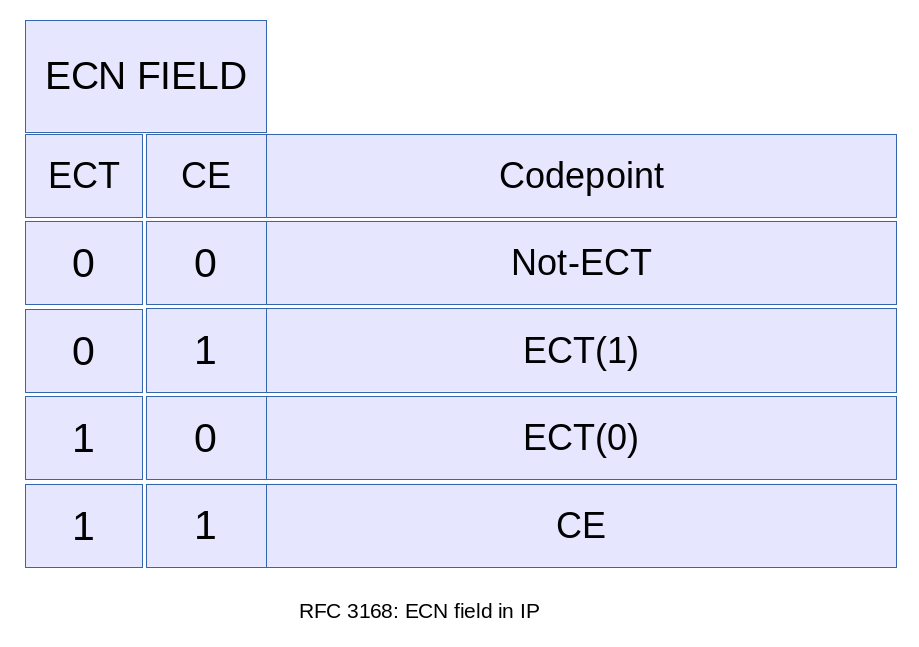
\includegraphics[width=0.30\textwidth]{Figures/iccps2014/ecn_field_in_ip.png}
  \caption{ECN Field In IP Header}
  \label{fig:ecn_field}
  \end{center}
\end{figure}

{\bf Gateways,} in the network maintain $Q_{min}$ and $Q_{max}$ thresholds for average queue size, $Q_{avg}$ for every
outgoing port. When a packet arrives at the gateway, one among the following actions is taken,

IF $Q_{min} \geq Q_{avg} \leq Q_{max}:$ Set ECN\_CE bit. 

IF $Q_{avg} < Q_{min}:$ Take no action.

IF $Q_{avg} > Q_{max}:$ Drop packet.

{\bf Receiver,} upon arrival of packet marked with ECN\_CE(Congestion experienced), sets a flag in the acknowledgment 
packet header and send it back to Sender.
{\bf Sender,} when receives this acknowledgment reduces the rate of transmission in order to avoid possible upcoming 
congestion. For example, in TCP, sender reduces the transmission rate by reducing its congestion window size and slow start threshold.
This mechanism avoids the unnecessary packet drops during mild congestion.

	Although there are modifications made to ECN as in~\cite{hadidraft}











